\documentclass[]{article}
\usepackage{lmodern}
\usepackage{amssymb,amsmath}
\usepackage{ifxetex,ifluatex}
\usepackage{fixltx2e} % provides \textsubscript
\ifnum 0\ifxetex 1\fi\ifluatex 1\fi=0 % if pdftex
  \usepackage[T1]{fontenc}
  \usepackage[utf8]{inputenc}
\else % if luatex or xelatex
  \ifxetex
    \usepackage{mathspec}
  \else
    \usepackage{fontspec}
  \fi
  \defaultfontfeatures{Ligatures=TeX,Scale=MatchLowercase}
\fi
% use upquote if available, for straight quotes in verbatim environments
\IfFileExists{upquote.sty}{\usepackage{upquote}}{}
% use microtype if available
\IfFileExists{microtype.sty}{%
\usepackage{microtype}
\UseMicrotypeSet[protrusion]{basicmath} % disable protrusion for tt fonts
}{}
\usepackage[margin=1in]{geometry}
\usepackage{hyperref}
\hypersetup{unicode=true,
            pdftitle={ex1},
            pdfauthor={Liav Alter},
            pdfborder={0 0 0},
            breaklinks=true}
\urlstyle{same}  % don't use monospace font for urls
\usepackage{color}
\usepackage{fancyvrb}
\newcommand{\VerbBar}{|}
\newcommand{\VERB}{\Verb[commandchars=\\\{\}]}
\DefineVerbatimEnvironment{Highlighting}{Verbatim}{commandchars=\\\{\}}
% Add ',fontsize=\small' for more characters per line
\usepackage{framed}
\definecolor{shadecolor}{RGB}{248,248,248}
\newenvironment{Shaded}{\begin{snugshade}}{\end{snugshade}}
\newcommand{\KeywordTok}[1]{\textcolor[rgb]{0.13,0.29,0.53}{\textbf{#1}}}
\newcommand{\DataTypeTok}[1]{\textcolor[rgb]{0.13,0.29,0.53}{#1}}
\newcommand{\DecValTok}[1]{\textcolor[rgb]{0.00,0.00,0.81}{#1}}
\newcommand{\BaseNTok}[1]{\textcolor[rgb]{0.00,0.00,0.81}{#1}}
\newcommand{\FloatTok}[1]{\textcolor[rgb]{0.00,0.00,0.81}{#1}}
\newcommand{\ConstantTok}[1]{\textcolor[rgb]{0.00,0.00,0.00}{#1}}
\newcommand{\CharTok}[1]{\textcolor[rgb]{0.31,0.60,0.02}{#1}}
\newcommand{\SpecialCharTok}[1]{\textcolor[rgb]{0.00,0.00,0.00}{#1}}
\newcommand{\StringTok}[1]{\textcolor[rgb]{0.31,0.60,0.02}{#1}}
\newcommand{\VerbatimStringTok}[1]{\textcolor[rgb]{0.31,0.60,0.02}{#1}}
\newcommand{\SpecialStringTok}[1]{\textcolor[rgb]{0.31,0.60,0.02}{#1}}
\newcommand{\ImportTok}[1]{#1}
\newcommand{\CommentTok}[1]{\textcolor[rgb]{0.56,0.35,0.01}{\textit{#1}}}
\newcommand{\DocumentationTok}[1]{\textcolor[rgb]{0.56,0.35,0.01}{\textbf{\textit{#1}}}}
\newcommand{\AnnotationTok}[1]{\textcolor[rgb]{0.56,0.35,0.01}{\textbf{\textit{#1}}}}
\newcommand{\CommentVarTok}[1]{\textcolor[rgb]{0.56,0.35,0.01}{\textbf{\textit{#1}}}}
\newcommand{\OtherTok}[1]{\textcolor[rgb]{0.56,0.35,0.01}{#1}}
\newcommand{\FunctionTok}[1]{\textcolor[rgb]{0.00,0.00,0.00}{#1}}
\newcommand{\VariableTok}[1]{\textcolor[rgb]{0.00,0.00,0.00}{#1}}
\newcommand{\ControlFlowTok}[1]{\textcolor[rgb]{0.13,0.29,0.53}{\textbf{#1}}}
\newcommand{\OperatorTok}[1]{\textcolor[rgb]{0.81,0.36,0.00}{\textbf{#1}}}
\newcommand{\BuiltInTok}[1]{#1}
\newcommand{\ExtensionTok}[1]{#1}
\newcommand{\PreprocessorTok}[1]{\textcolor[rgb]{0.56,0.35,0.01}{\textit{#1}}}
\newcommand{\AttributeTok}[1]{\textcolor[rgb]{0.77,0.63,0.00}{#1}}
\newcommand{\RegionMarkerTok}[1]{#1}
\newcommand{\InformationTok}[1]{\textcolor[rgb]{0.56,0.35,0.01}{\textbf{\textit{#1}}}}
\newcommand{\WarningTok}[1]{\textcolor[rgb]{0.56,0.35,0.01}{\textbf{\textit{#1}}}}
\newcommand{\AlertTok}[1]{\textcolor[rgb]{0.94,0.16,0.16}{#1}}
\newcommand{\ErrorTok}[1]{\textcolor[rgb]{0.64,0.00,0.00}{\textbf{#1}}}
\newcommand{\NormalTok}[1]{#1}
\usepackage{graphicx,grffile}
\makeatletter
\def\maxwidth{\ifdim\Gin@nat@width>\linewidth\linewidth\else\Gin@nat@width\fi}
\def\maxheight{\ifdim\Gin@nat@height>\textheight\textheight\else\Gin@nat@height\fi}
\makeatother
% Scale images if necessary, so that they will not overflow the page
% margins by default, and it is still possible to overwrite the defaults
% using explicit options in \includegraphics[width, height, ...]{}
\setkeys{Gin}{width=\maxwidth,height=\maxheight,keepaspectratio}
\IfFileExists{parskip.sty}{%
\usepackage{parskip}
}{% else
\setlength{\parindent}{0pt}
\setlength{\parskip}{6pt plus 2pt minus 1pt}
}
\setlength{\emergencystretch}{3em}  % prevent overfull lines
\providecommand{\tightlist}{%
  \setlength{\itemsep}{0pt}\setlength{\parskip}{0pt}}
\setcounter{secnumdepth}{0}
% Redefines (sub)paragraphs to behave more like sections
\ifx\paragraph\undefined\else
\let\oldparagraph\paragraph
\renewcommand{\paragraph}[1]{\oldparagraph{#1}\mbox{}}
\fi
\ifx\subparagraph\undefined\else
\let\oldsubparagraph\subparagraph
\renewcommand{\subparagraph}[1]{\oldsubparagraph{#1}\mbox{}}
\fi

%%% Use protect on footnotes to avoid problems with footnotes in titles
\let\rmarkdownfootnote\footnote%
\def\footnote{\protect\rmarkdownfootnote}

%%% Change title format to be more compact
\usepackage{titling}

% Create subtitle command for use in maketitle
\providecommand{\subtitle}[1]{
  \posttitle{
    \begin{center}\large#1\end{center}
    }
}

\setlength{\droptitle}{-2em}

  \title{ex1}
    \pretitle{\vspace{\droptitle}\centering\huge}
  \posttitle{\par}
    \author{Liav Alter}
    \preauthor{\centering\large\emph}
  \postauthor{\par}
    \date{}
    \predate{}\postdate{}
  

\begin{document}
\maketitle

Thanks

\subsubsection{Pisa Test}\label{pisa-test}

\paragraph{1.1}\label{section}

First we will want to load our Pisa test excel files. To do that, we'll
define our work directory to be the folder that contains the `pisa.xlsx'
file, with the command wordkir. As the `pisa.xlsx' contains 3 sheets, we
will load each of them to a different reference.

\begin{Shaded}
\begin{Highlighting}[]
\NormalTok{workdir =}\StringTok{ "C:/Users/Liav/Desktop/Uni/R/targil1"}
\KeywordTok{setwd}\NormalTok{(workdir)}

\NormalTok{pisa_math =}\StringTok{ }\KeywordTok{read_excel}\NormalTok{(}\StringTok{"pisa.xlsx"}\NormalTok{, }\DataTypeTok{sheet=}\DecValTok{1}\NormalTok{)}

\NormalTok{pisa_reading =}\StringTok{ }\KeywordTok{read_excel}\NormalTok{(}\StringTok{"pisa.xlsx"}\NormalTok{, }\DataTypeTok{sheet=}\DecValTok{2}\NormalTok{)}
\NormalTok{pisa_science =}\StringTok{ }\KeywordTok{read_excel}\NormalTok{(}\StringTok{"pisa.xlsx"}\NormalTok{, }\DataTypeTok{sheet=}\DecValTok{3}\NormalTok{)}
\end{Highlighting}
\end{Shaded}

To get a clue about how the data looks like, we can use the head command
to pring the first rows of it. Let's make an example with pisa\_math.

\begin{Shaded}
\begin{Highlighting}[]
\KeywordTok{head}\NormalTok{(pisa_math)}
\end{Highlighting}
\end{Shaded}

\begin{verbatim}
## # A tibble: 6 x 3
##   Country                      Score  year
##   <chr>                        <chr> <dbl>
## 1 International Average (OECD) 490    2015
## 2  Albania                     413    2015
## 3  Algeria                     360    2015
## 4  Argentina                   409    2015
## 5  Australia                   494    2015
## 6  Austria                     497    2015
\end{verbatim}

Since all the worksheets share the same columns names, to differ them,
we can change some of the columns name.

\begin{Shaded}
\begin{Highlighting}[]
\KeywordTok{colnames}\NormalTok{(pisa_math)[}\DecValTok{2}\NormalTok{] =}\StringTok{ "math_score"}
\KeywordTok{colnames}\NormalTok{(pisa_reading)[}\DecValTok{2}\NormalTok{] =}\StringTok{ "reading_score"}
\KeywordTok{colnames}\NormalTok{(pisa_science)[}\DecValTok{2}\NormalTok{] =}\StringTok{ "science_score"}  
\end{Highlighting}
\end{Shaded}

\paragraph{1.2}\label{section-1}

We would like to check who were the leading countries in every field in
2015. To do so, we will sort by descending order the 2015 year subset.
This command might seem very complicated, let's try to explain it
simply:

\begin{enumerate}
\def\labelenumi{\arabic{enumi}.}
\item
  head command (x, n= 3L) is the same head command we used before, but
  now we used ``n=3L'' to get the first 3 lines.
\item
  pisa\_math{[}y, year=2015{]} command gives us a susbet of the
  pisa\_math rows that their value in column `year' equals to 2015.
  notice that pisa\_math is the name of the dataframe, we can change it
  later to another name for the other dataframes.
\item
  order(pisa\_math\$math\_score, decreasing = TRUE) returns the data
  decreasing order if the data frame be the pisa\_math column.
\end{enumerate}

To connect those three simple functions we can write the 3rd function
instead of y, and the joined 2nd function (with 3 insted of y) instead
of x, and now we got the 3 first countries orederd by scores, only when
year was 2015.

\begin{Shaded}
\begin{Highlighting}[]
\KeywordTok{head}\NormalTok{(}\KeywordTok{subset}\NormalTok{(pisa_math[}\KeywordTok{order}\NormalTok{(pisa_math}\OperatorTok{$}\NormalTok{math_score, }\DataTypeTok{decreasing =} \OtherTok{TRUE}\NormalTok{), ], year }\OperatorTok{==}\StringTok{ }\DecValTok{2015}\NormalTok{), }\DataTypeTok{n=}\NormalTok{3L)}
\end{Highlighting}
\end{Shaded}

\begin{verbatim}
## # A tibble: 3 x 3
##   Country           math_score  year
##   <chr>             <chr>      <dbl>
## 1  Singapore        564         2015
## 2  Hong Kong, China 548         2015
## 3  Macau            544         2015
\end{verbatim}

\begin{Shaded}
\begin{Highlighting}[]
\KeywordTok{head}\NormalTok{(}\KeywordTok{subset}\NormalTok{(pisa_science[}\KeywordTok{order}\NormalTok{(pisa_science}\OperatorTok{$}\NormalTok{science_score, }\DataTypeTok{decreasing =} \OtherTok{TRUE}\NormalTok{), ], year }\OperatorTok{==}\StringTok{ }\DecValTok{2015}\NormalTok{), }\DataTypeTok{n=}\NormalTok{3L)}
\end{Highlighting}
\end{Shaded}

\begin{verbatim}
## # A tibble: 3 x 3
##   Country    science_score  year
##   <chr>      <chr>         <dbl>
## 1  Singapore 556            2015
## 2  Japan     538            2015
## 3  Estonia   534            2015
\end{verbatim}

\begin{Shaded}
\begin{Highlighting}[]
\KeywordTok{head}\NormalTok{(}\KeywordTok{subset}\NormalTok{(pisa_reading[}\KeywordTok{order}\NormalTok{(pisa_reading}\OperatorTok{$}\NormalTok{reading_score, }\DataTypeTok{decreasing =} \OtherTok{TRUE}\NormalTok{), ], year }\OperatorTok{==}\StringTok{ }\DecValTok{2015}\NormalTok{), }\DataTypeTok{n=}\NormalTok{3L)}
\end{Highlighting}
\end{Shaded}

\begin{verbatim}
## # A tibble: 3 x 3
##   Country           reading_score  year
##   <chr>             <chr>         <dbl>
## 1  Singapore        535            2015
## 2  Canada           527            2015
## 3  Hong Kong, China 527            2015
\end{verbatim}

We can see that Singapore students has the best Pisa test grades in
2015, in all fields.

\paragraph{1.3}\label{section-2}

To continue working on this data set, we would like to merge the all
three dataframes to one. For this, we can use the merge command. At
first we merge the science and math grades columns. The command
``all=TRUE'' used to keep the NA value rows. The ``sort=TRUE'' command
used to keep the new dataframe sorted by the country name.

After we merged science and math grade we can merge them again to the
reading grade dataframe by the same method.

\begin{Shaded}
\begin{Highlighting}[]
\NormalTok{data =}\StringTok{ }\KeywordTok{merge}\NormalTok{( }\KeywordTok{merge}\NormalTok{( pisa_math, pisa_science, }\DataTypeTok{by =} \KeywordTok{c}\NormalTok{(}\StringTok{"Country"}\NormalTok{,}\StringTok{"year"}\NormalTok{) ,}\DataTypeTok{all =} \OtherTok{TRUE}\NormalTok{, }\DataTypeTok{sort =} \OtherTok{TRUE}\NormalTok{), pisa_reading, }\DataTypeTok{by =} \KeywordTok{c}\NormalTok{(}\StringTok{"Country"}\NormalTok{,}\StringTok{"year"}\NormalTok{), }\DataTypeTok{all =} \OtherTok{TRUE}\NormalTok{, }\DataTypeTok{sort=}\OtherTok{TRUE}\NormalTok{ )}
\end{Highlighting}
\end{Shaded}

Here is ther head of our new merged dataframe:

\begin{verbatim}
##         Country year math_score science_score reading_score
## 1   Switzerland 2000       <NA>          <NA>           494
## 2   Switzerland 2003        527          <NA>           499
## 3   Switzerland 2006        530           512           499
## 4   Switzerland 2009        534           517           501
## 5   Switzerland 2012        531           515           509
## 6   Switzerland 2015        521           506           492
## 7       Albania 2000       <NA>          <NA>           349
\end{verbatim}

Before we continue to answer the next questions, we would like to make
sure that the columns type is still numeric, so we can apply arithmetic
functions on them. For that, we'll use the following:

\begin{Shaded}
\begin{Highlighting}[]
\KeywordTok{sapply}\NormalTok{(data, class)}
\end{Highlighting}
\end{Shaded}

\begin{verbatim}
##       Country          year    math_score science_score reading_score 
##   "character"     "numeric"   "character"   "character"   "character"
\end{verbatim}

We can see that the type of the values in the score columns are
character. There for, we'll use sapply to apply the function as numeric
on the 3rd to 5th columns.

\begin{Shaded}
\begin{Highlighting}[]
\NormalTok{data[, }\DecValTok{3}\OperatorTok{:}\DecValTok{5}\NormalTok{] <-}\StringTok{ }\KeywordTok{sapply}\NormalTok{(data[, }\DecValTok{3}\OperatorTok{:}\DecValTok{5}\NormalTok{], as.numeric)}
\KeywordTok{sapply}\NormalTok{(data, class)}
\end{Highlighting}
\end{Shaded}

\begin{verbatim}
##       Country          year    math_score science_score reading_score 
##   "character"     "numeric"     "numeric"     "numeric"     "numeric"
\end{verbatim}

And now we can see the type changed to numeric.

\paragraph{1.4}\label{section-3}

We'll check the avarage pisa scores (average of all three fields scores)
for each country on every year. To make it a fair competition, we will
calculate only the rows that includes all three grades.

\begin{Shaded}
\begin{Highlighting}[]
\NormalTok{data}\OperatorTok{$}\NormalTok{average_score <-}\StringTok{ }\KeywordTok{rowMeans}\NormalTok{(data[,}\DecValTok{3}\OperatorTok{:}\DecValTok{5}\NormalTok{], }\DataTypeTok{na.rm=}\OtherTok{TRUE}\NormalTok{)}
\end{Highlighting}
\end{Shaded}

Here is ther head of our new dataframe, with the average column:

\begin{verbatim}
##         Country year math_score science_score reading_score average_score
## 1   Switzerland 2000         NA            NA           494      494.0000
## 2   Switzerland 2003        527            NA           499      513.0000
## 3   Switzerland 2006        530           512           499      513.6667
\end{verbatim}

\paragraph{1.5}\label{section-4}

As beofre, let's use the subset and order functions to present the top
average scores countries in 2006 and 2015. This time, we will use
``{[},c(1,6){]}'' slicing to show only the 1st, 2nd and 6th column.

\begin{Shaded}
\begin{Highlighting}[]
\KeywordTok{head}\NormalTok{(}\KeywordTok{subset}\NormalTok{(data[}\KeywordTok{order}\NormalTok{(data}\OperatorTok{$}\NormalTok{average_score, }\DataTypeTok{decreasing =} \OtherTok{TRUE}\NormalTok{), ], year }\OperatorTok{==}\StringTok{ }\DecValTok{2015}\NormalTok{)[,}\KeywordTok{c}\NormalTok{(}\DecValTok{1}\NormalTok{,}\DecValTok{2}\NormalTok{,}\DecValTok{6}\NormalTok{)], }\DataTypeTok{n=}\NormalTok{3L)}
\end{Highlighting}
\end{Shaded}

\begin{verbatim}
##               Country year average_score
## 348         Singapore 2015      551.6667
## 162  Hong Kong, China 2015      532.6667
## 204             Japan 2015      528.6667
\end{verbatim}

\begin{Shaded}
\begin{Highlighting}[]
\KeywordTok{head}\NormalTok{(}\KeywordTok{subset}\NormalTok{(data[}\KeywordTok{order}\NormalTok{(data}\OperatorTok{$}\NormalTok{average_score, }\DataTypeTok{decreasing =} \OtherTok{TRUE}\NormalTok{), ], year }\OperatorTok{==}\StringTok{ }\DecValTok{2006}\NormalTok{)[,}\KeywordTok{c}\NormalTok{(}\DecValTok{1}\NormalTok{,}\DecValTok{2}\NormalTok{,}\DecValTok{6}\NormalTok{)], }\DataTypeTok{n=}\NormalTok{3L)}
\end{Highlighting}
\end{Shaded}

\begin{verbatim}
##               Country year average_score
## 129           Finland 2006      552.6667
## 159  Hong Kong, China 2006      541.6667
## 363       South Korea 2006      541.6667
\end{verbatim}

\begin{center}\rule{0.5\linewidth}{\linethickness}\end{center}

\subsubsection{Salaries}\label{salaries}

Now, we'll start working on the salaries file.

2.1 From a brief look on the data, we can see that the 2nd sheet on the
sal.xlsx file is just an addition of a nonimnal salary column. Therefor,
to save time and code, it will be a good idea to join the two dataframes
by adding the ``current'' column from the 2nd dataframe to the first
one. We' will use the same read\_excel command from before to do so, and
than we'll just add manually the missing column.

\begin{Shaded}
\begin{Highlighting}[]
\NormalTok{salaries =}\StringTok{ }\KeywordTok{read_excel}\NormalTok{(}\StringTok{"sal.xlsx"}\NormalTok{, }\DataTypeTok{sheet=}\DecValTok{1}\NormalTok{)}
\NormalTok{sal_nominal =}\StringTok{ }\KeywordTok{read_excel}\NormalTok{(}\StringTok{"sal.xlsx"}\NormalTok{, }\DataTypeTok{sheet=}\DecValTok{2}\NormalTok{)   }
\NormalTok{salaries}\OperatorTok{$}\NormalTok{current =}\StringTok{ }\NormalTok{sal_nominal}\OperatorTok{$}\NormalTok{current}
\end{Highlighting}
\end{Shaded}

Here are some rows of our new dataframe:

\begin{verbatim}
## # A tibble: 3 x 16
##   TIME  `2000` `2005` `2006` `2007` `2008` `2009` `2010` `2011` `2012`
##   <chr>  <dbl>  <dbl>  <dbl>  <dbl>  <dbl>  <dbl>  <dbl>  <dbl>  <dbl>
## 1  Por~     NA    100     98     96     95     97     98    100     86
## 2  Spa~     NA    100    101     99    103    106    106    100     95
## 3  Swe~     NA    100     NA    103     NA    104     NA    103     NA
## # ... with 6 more variables: `2013` <dbl>, `2014` <dbl>, `2015` <dbl>,
## #   `2016` <dbl>, `2017` <dbl>, current <dbl>
\end{verbatim}

\paragraph{Data complection and
cleaning}\label{data-complection-and-cleaning}

Before we will start analyzing our data, we will want to have a look of
it and see if there are missing values or any outliners that we need to
take care of. After a quick look on the salaries dataframe, we can see
that some of the salaries are missing. Take a look for example, on the
2006 and 2008 salary in Sweden. In order to fill the missing data, we
can user linear regression and try to predict what were the salaries in
the missing fields.

To fill out dataframe, I wrote myself the following function:

\begin{Shaded}
\begin{Highlighting}[]
\NormalTok{salary_predict <-}\StringTok{ }\ControlFlowTok{function}\NormalTok{(row, i) \{}
\NormalTok{df <-}\StringTok{ }\KeywordTok{data.frame}\NormalTok{(}\DataTypeTok{x=}\DecValTok{1}\OperatorTok{:}\DecValTok{13}\NormalTok{,}\DataTypeTok{y=}\DecValTok{100}\OperatorTok{*}\NormalTok{(}\DecValTok{1}\OperatorTok{:}\DecValTok{13}\NormalTok{))}
\NormalTok{df}\OperatorTok{$}\NormalTok{y =}\StringTok{ }\KeywordTok{as.vector}\NormalTok{(}\KeywordTok{unlist}\NormalTok{(salaries[i,}\DecValTok{3}\OperatorTok{:}\DecValTok{15}\NormalTok{]))}
\NormalTok{df}\OperatorTok{$}\NormalTok{x=}\StringTok{ }\KeywordTok{as.numeric}\NormalTok{(}\KeywordTok{colnames}\NormalTok{(salaries[}\DecValTok{3}\OperatorTok{:}\DecValTok{15}\NormalTok{]))}
\NormalTok{model <-}\StringTok{ }\KeywordTok{lm}\NormalTok{(y}\OperatorTok{~}\NormalTok{x}\OperatorTok{+}\DecValTok{1}\NormalTok{,}\DataTypeTok{data=}\NormalTok{df)}
\NormalTok{df}\OperatorTok{$}\NormalTok{y_hat <-}\StringTok{ }\KeywordTok{predict.lm}\NormalTok{(model, }\DataTypeTok{newdata =}\NormalTok{ df)}
\NormalTok{df=}\StringTok{ }\NormalTok{df }\OperatorTok\StringTok{ }\KeywordTok{mutate}\NormalTok{(}\DataTypeTok{y =} \KeywordTok{ifelse}\NormalTok{(}\KeywordTok{is.na}\NormalTok{(y), y_hat, y))}
\KeywordTok{return}\NormalTok{(df}\OperatorTok{$}\NormalTok{y)}
\NormalTok{\}}
\end{Highlighting}
\end{Shaded}

The function parameters are a row, and a row index. Since i wanted to
predict more efficiently the missing values from years 2005-2017, and
since later on we will not need it, i decided to ignore the ``2000''
column for now. The function creates a new dataframe with index values
for cells. Afterwards, save inside them the Y vector which we want to
predict (our explained variable), which in our case is the row's 3rd to
15th values, which we had to unlist them and save as vector because of
the predict function input demands. We did the same for our explaining
variable, which is the series of years 2005-2017. model function creates
a model, and y\_hat is the vector of model predictions. Since we already
have some data, we will take only the missing index and mutate them into
our Y vector.

After we built the function, we will have to apply them on each row. For
this, we can use a for loop that go through each row and replacing the
values 3:15 in the function output.

\begin{Shaded}
\begin{Highlighting}[]
\ControlFlowTok{for}\NormalTok{(i }\ControlFlowTok{in} \DecValTok{1}\OperatorTok{:}\KeywordTok{nrow}\NormalTok{(salaries)) \{}
\NormalTok{    row <-}\StringTok{ }\NormalTok{salaries[i,]}
\NormalTok{    salaries[i,}\DecValTok{3}\OperatorTok{:}\DecValTok{15}\NormalTok{] =}\StringTok{  }\KeywordTok{salary_predict}\NormalTok{(row,i)}
\NormalTok{\}}
\end{Highlighting}
\end{Shaded}

And here is an example our filled data:

\begin{verbatim}
## # A tibble: 3 x 15
##   TIME  `2005` `2006` `2007` `2008` `2009` `2010` `2011` `2012` `2013`
##   <chr>  <dbl>  <dbl>  <dbl>  <dbl>  <dbl>  <dbl>  <dbl>  <dbl>  <dbl>
## 1  Por~    100   98       96    95      97    98     100    86      84
## 2  Spa~    100  101       99   103     106   106     100    95      92
## 3  Swe~    100   99.3    103   103.    104   106.    103   110.    108
## # ... with 5 more variables: `2014` <dbl>, `2015` <dbl>, `2016` <dbl>,
## #   `2017` <dbl>, current <dbl>
\end{verbatim}

\subparagraph{Note: Since our next question will be about years
2005-2017, i decided to drop 2000 salaries for
now.}\label{note-since-our-next-question-will-be-about-years-2005-2017-i-decided-to-drop-2000-salaries-for-now.}

\paragraph{2.2}\label{section-5}

Now, we can find the nominal wages in each country in any year, by using
the ``current'' column. Since the wage from 2006 to 2016. The forumla is
going to be (Year.i*year.0)/nominal, while year 0 is 2017. To do this,
we will use for a for loop again, this time on columns 2:13 (since the
13th column is 2017 wage)

\begin{Shaded}
\begin{Highlighting}[]
\ControlFlowTok{for}\NormalTok{(i }\ControlFlowTok{in} \DecValTok{2}\OperatorTok{:}\KeywordTok{ncol}\NormalTok{(salaries)) \{}
\NormalTok{  salaries[i] =}\StringTok{ }\NormalTok{((salaries[i]}\OperatorTok{/}\NormalTok{salaries}\OperatorTok{$}\StringTok{`}\DataTypeTok{2017}\StringTok{`}\NormalTok{)}\OperatorTok{*}\NormalTok{salaries}\OperatorTok{$}\NormalTok{current)}
\NormalTok{\}}
\NormalTok{salaries[}\DecValTok{16}\OperatorTok{:}\DecValTok{18}\NormalTok{,]}
\end{Highlighting}
\end{Shaded}

\begin{verbatim}
## # A tibble: 3 x 15
##   TIME  `2005` `2006` `2007` `2008` `2009` `2010` `2011` `2012` `2013`
##   <chr>  <dbl>  <dbl>  <dbl>  <dbl>  <dbl>  <dbl>  <dbl>  <dbl>  <dbl>
## 1  Por~ 43633. 42760. 41887. 41451. 42324. 42760. 43633. 37524. 36651.
## 2  Spa~ 52827. 53355. 52299. 54412. 55997. 55997. 52827. 50186. 48601.
## 3  Swe~ 35487. 35230. 36551. 36478. 36906. 37727. 36551. 38975. 38326.
## # ... with 5 more variables: `2014` <dbl>, `2015` <dbl>, `2016` <dbl>,
## #   `2017` <dbl>, current <dbl>
\end{verbatim}

Since Estonoia current wage in nominal terms is missing, , we got NA
over the values. Since this row can help us at the moment, we can drop
the Estonia salary row. We can also drop the nominal current salary,
since it equals to the 2017 salary

\begin{verbatim}
## # A tibble: 1 x 14
##   TIME  `2005` `2006` `2007` `2008` `2009` `2010` `2011` `2012` `2013`
##   <chr>  <dbl>  <dbl>  <dbl>  <dbl>  <dbl>  <dbl>  <dbl>  <dbl>  <dbl>
## 1  Est~     NA     NA     NA     NA     NA     NA     NA     NA     NA
## # ... with 4 more variables: `2014` <dbl>, `2015` <dbl>, `2016` <dbl>,
## #   `2017` <dbl>
\end{verbatim}

\subsubsection{Data analyzing}\label{data-analyzing}

\paragraph{2.3}\label{section-6}

To check the relative of a country from the rest of the world, we can
add an average international rating row for each year. We'll it (OECD
(Average International). To do so, we will create a vector with the row
means, and add the title of it manually. Afterwords, we can add it
manually to salaries dataframe.

\begin{Shaded}
\begin{Highlighting}[]
\NormalTok{row_name =}\StringTok{ "International Average (OECD)"}
\NormalTok{avg_vec =}\StringTok{ }\KeywordTok{c}\NormalTok{(row_name, }\KeywordTok{colMeans}\NormalTok{(salaries[}\DecValTok{2}\OperatorTok{:}\KeywordTok{ncol}\NormalTok{(salaries)]))}
\end{Highlighting}
\end{Shaded}

Now, we can join them together with the rbind command. We will use
head(salaries) command to check out the top of our data as we did
before.

\begin{Shaded}
\begin{Highlighting}[]
\NormalTok{salaries <-}\StringTok{ }\KeywordTok{rbind}\NormalTok{(avg_vec, salaries)}
\KeywordTok{colnames}\NormalTok{(salaries)[}\DecValTok{1}\NormalTok{] <-}\StringTok{ "Country"}
\KeywordTok{head}\NormalTok{(salaries)}
\end{Highlighting}
\end{Shaded}

\begin{verbatim}
## # A tibble: 6 x 14
##   Country `2005` `2006` `2007` `2008` `2009` `2010` `2011` `2012` `2013`
##   <chr>   <chr>  <chr>  <chr>  <chr>  <chr>  <chr>  <chr>  <chr>  <chr> 
## 1 Intern~ 42590~ 42951~ 43062~ 43569~ 44379~ 44562~ 44183~ 43784~ 43763~
## 2  Austr~ 51322~ 50295~ 51322~ 53374~ 52861~ 53888~ 54914~ 54914~ 56967~
## 3  Austr~ 49334~ 49334~ 49827~ 49827~ 50814~ 51307~ 50814~ 50321~ 49827~
## 4  Denma~ 52535~ 53060~ 53060~ 54111~ 57263~ 56212~ 55162~ 53586~ 54636~
## 5  Finla~ 43893~ 45210~ 45210~ 46088~ 46088~ 46966~ 46527~ 45649~ 45210~
## 6  France 39396~ 39396~ 39002~ 38214~ 38214~ 38608~ 38214~ 37820~ 37426~
## # ... with 4 more variables: `2014` <chr>, `2015` <chr>, `2016` <chr>,
## #   `2017` <chr>
\end{verbatim}

\paragraph{2.4}\label{section-7}

Now we can, for example, analyse year 2010. Let's check which salary was
the closest to the average in 2010, and check which one was the most far
from it (from both under and above) To do so, we will go throguh the
following levels: 1. Create a reference with the salaries\$`2010' values
2. Reduce from it the OCED (remember that this is the first row now),
and get the absolut value of to get only the distance. 3. The maximum
and minimum of the original are the most far values from average, and
the minumim of the absolut value reduced column is the closest to
average.

Notice that on the `which' command (that returns the index that inside
the brackets) we add +1 to the index because we sliced the
salaries\$2010 vector

\begin{Shaded}
\begin{Highlighting}[]
\NormalTok{column =}\StringTok{ }\KeywordTok{as.numeric}\NormalTok{(salaries}\OperatorTok{$}\StringTok{`}\DataTypeTok{2010}\StringTok{`}\NormalTok{)}
\NormalTok{salaries[}\KeywordTok{which}\NormalTok{(salaries}\OperatorTok{$}\StringTok{`}\DataTypeTok{2010}\StringTok{`}\OperatorTok{==}\KeywordTok{max}\NormalTok{(column)),]}
\end{Highlighting}
\end{Shaded}

\begin{verbatim}
## # A tibble: 1 x 14
##   Country `2005` `2006` `2007` `2008` `2009` `2010` `2011` `2012` `2013`
##   <chr>    <dbl>  <dbl>  <dbl>  <dbl>  <dbl>  <dbl>  <dbl>  <dbl>  <dbl>
## 1  Luxem~ 94924. 94924. 94924. 1.02e5 1.08e5 1.06e5 1.03e5 1.06e5 1.07e5
## # ... with 4 more variables: `2014` <dbl>, `2015` <dbl>, `2016` <dbl>,
## #   `2017` <dbl>
\end{verbatim}

\begin{Shaded}
\begin{Highlighting}[]
\NormalTok{salaries[}\KeywordTok{which}\NormalTok{(salaries}\OperatorTok{$}\StringTok{`}\DataTypeTok{2010}\StringTok{`}\OperatorTok{==}\KeywordTok{min}\NormalTok{(column)),]}
\end{Highlighting}
\end{Shaded}

\begin{verbatim}
## # A tibble: 1 x 14
##   Country `2005` `2006` `2007` `2008` `2009` `2010` `2011` `2012` `2013`
##   <chr>    <dbl>  <dbl>  <dbl>  <dbl>  <dbl>  <dbl>  <dbl>  <dbl>  <dbl>
## 1  Hunga~ 18744. 18370. 17620. 17245. 15370. 14808. 14246. 13309. 12746.
## # ... with 4 more variables: `2014` <dbl>, `2015` <dbl>, `2016` <dbl>,
## #   `2017` <dbl>
\end{verbatim}

\begin{Shaded}
\begin{Highlighting}[]
\NormalTok{salaries[}\KeywordTok{which}\NormalTok{ (}\KeywordTok{abs}\NormalTok{(column[}\DecValTok{2}\OperatorTok{:}\KeywordTok{nrow}\NormalTok{(salaries)]}\OperatorTok{-}\NormalTok{column[}\DecValTok{1}\NormalTok{]) }\OperatorTok{==}\StringTok{ }\KeywordTok{min}\NormalTok{(}\KeywordTok{abs}\NormalTok{(column[}\DecValTok{2}\OperatorTok{:}\KeywordTok{nrow}\NormalTok{(salaries)]}\OperatorTok{-}\NormalTok{column[}\DecValTok{1}\NormalTok{])))}\OperatorTok{+}\DecValTok{1}\NormalTok{,]}
\end{Highlighting}
\end{Shaded}

\begin{verbatim}
## # A tibble: 1 x 14
##   Country `2005` `2006` `2007` `2008` `2009` `2010` `2011` `2012` `2013`
##   <chr>    <dbl>  <dbl>  <dbl>  <dbl>  <dbl>  <dbl>  <dbl>  <dbl>  <dbl>
## 1  Portu~ 43633. 42760. 41887. 41451. 42324. 42760. 43633. 37524. 36651.
## # ... with 4 more variables: `2014` <dbl>, `2015` <dbl>, `2016` <dbl>,
## #   `2017` <dbl>
\end{verbatim}

We got that the highest salary was at Luxembourg, the lowest was in at
Hungary, and the closest to average Portugal

\paragraph{2.5}\label{section-8}

Here are the highest earned countries in 2015.

\begin{Shaded}
\begin{Highlighting}[]
\KeywordTok{head}\NormalTok{(}\KeywordTok{subset}\NormalTok{(salaries[}\KeywordTok{order}\NormalTok{(salaries}\OperatorTok{$}\StringTok{`}\DataTypeTok{2015}\StringTok{`}\NormalTok{, }\DataTypeTok{decreasing =} \OtherTok{TRUE}\NormalTok{), }\KeywordTok{c}\NormalTok{(}\DecValTok{1}\NormalTok{,}\DecValTok{12}\NormalTok{)]), }\DataTypeTok{n=}\NormalTok{5L)}
\end{Highlighting}
\end{Shaded}

\begin{verbatim}
## # A tibble: 5 x 2
##   Country         `2015`
##   <chr>            <dbl>
## 1  Luxembourg    110112.
## 2  Germany        73978.
## 3  United States  63184.
## 4  Ireland        58953.
## 5  Australia      58507.
\end{verbatim}

Let's check their rank in the Pisa test.

\begin{Shaded}
\begin{Highlighting}[]
\NormalTok{twenty_fifteen =}\StringTok{ }\NormalTok{data[}\KeywordTok{which}\NormalTok{(data}\OperatorTok{$}\NormalTok{year}\OperatorTok{==}\DecValTok{2015}\NormalTok{),]}
\NormalTok{twenty_fifteen =}\StringTok{ }\KeywordTok{merge}\NormalTok{( salaries[(}\KeywordTok{which}\NormalTok{(}\KeywordTok{colnames}\NormalTok{(salaries)}\OperatorTok{==}\KeywordTok{c}\NormalTok{(}\StringTok{"Country"}\NormalTok{,}\StringTok{"2015"}\NormalTok{)))], twenty_fifteen, }\DataTypeTok{by =} \KeywordTok{c}\NormalTok{(}\StringTok{"Country"}\NormalTok{) ,}\DataTypeTok{all =} \OtherTok{TRUE}\NormalTok{, }\DataTypeTok{sort =} \OtherTok{TRUE}\NormalTok{)}
\KeywordTok{head}\NormalTok{(twenty_fifteen[}\KeywordTok{order}\NormalTok{(twenty_fifteen}\OperatorTok{$}\StringTok{`}\DataTypeTok{2015}\StringTok{`}\NormalTok{, }\DataTypeTok{decreasing =} \OtherTok{TRUE}\NormalTok{),],}\DataTypeTok{n =} \DecValTok{5}\NormalTok{)}
\end{Highlighting}
\end{Shaded}

\begin{verbatim}
##           Country      2015 year math_score science_score reading_score
## 41     Luxembourg 110111.54 2015        486           483           481
## 25        Germany  73977.59 2015        506           509           509
## 71  United States  63184.36 2015        470           496           497
## 31        Ireland  58952.52 2015        504           503           521
## 6       Australia  58507.16 2015        494           510           503
##    average_score
## 41      483.3333
## 25      508.0000
## 71      487.6667
## 31      509.3333
## 6       502.3333
\end{verbatim}

We can see that there is no high correlation between the salaries in
2015 to the Pisa scores.

\paragraph{2.6}\label{section-9}

Let's check the change in salary between 2005 and 2017. To do so, we can
copy the 2005, 2017 columns to a new dataframe and calculate the percent
of change. Afterwards we can use the head and order function to show the
top 5, as we did before.

\begin{Shaded}
\begin{Highlighting}[]
\NormalTok{changes =}\StringTok{ }\NormalTok{salaries[}\KeywordTok{c}\NormalTok{(}\DecValTok{1}\NormalTok{,}\DecValTok{2}\NormalTok{,}\KeywordTok{ncol}\NormalTok{(salaries))]}
\NormalTok{changes}\OperatorTok{$}\NormalTok{change =}\StringTok{ }\NormalTok{(changes}\OperatorTok{$}\StringTok{`}\DataTypeTok{2017}\StringTok{`}\OperatorTok{/}\NormalTok{changes}\OperatorTok{$}\StringTok{`}\DataTypeTok{2005}\StringTok{`}\NormalTok{)}\OperatorTok{*}\DecValTok{100}
\KeywordTok{head}\NormalTok{(changes[}\KeywordTok{order}\NormalTok{(changes}\OperatorTok{$}\NormalTok{change, }\DataTypeTok{decreasing =} \OtherTok{TRUE}\NormalTok{),],}\DataTypeTok{n =} \DecValTok{5}\NormalTok{)}
\end{Highlighting}
\end{Shaded}

\begin{verbatim}
## # A tibble: 5 x 4
##   Country `2005` `2017` change
##   <chr>    <dbl>  <dbl>  <dbl>
## 1  Latvia 13716. 19696.   144.
## 2  Israel 23367. 33442.   143.
## 3  Poland 20433. 25553.   125.
## 4  Mexico 32478. 40595.   125.
## 5  Sweden 35487. 43827.   124.
\end{verbatim}

We can see that Latvia has the biggest growth in the teachers salary,
and right after, Israel. One reason to that might be the an increase in
the price index or inflation

\subsection{Salaries vs.~Test grades}\label{salaries-vs.test-grades}

\paragraph{3.1}\label{section-10}

To check the influence of the salaries on the test grades, let us first
merge our two data set and drop the NA values. To do so, we first need
to gather the data. To do so we will use the command gather from
``tidyr'' library. gather() arguments are first, the name of the
dataframe, second, the name you want for you new category column (that's
called the key), and third is the name you want for your new value
column (called value). After that are any column that you want to gather
into the new key and value columns.Because we want all the year columns
gathered but not the country columns, we will add the argument
``-Country'' (pay attention to the minus sign).

After we gathered the data, we can easily merge it to the grades data,
since now their shape is similar. notice that rows that aren't filled in
both dataframes are removed automatically.

In addition, we use the same functions as before to get the OECD average
grades of each year. Notice that some of them are missing values, i
decided to drop them.

Let's have a look on the gathered salaries dataframe:

\begin{Shaded}
\begin{Highlighting}[]
\NormalTok{gathered_salaries =}\StringTok{ }\KeywordTok{gather}\NormalTok{(}\DataTypeTok{data =}\NormalTok{ salaries, }\DataTypeTok{key =} \StringTok{"year"}\NormalTok{, }\DataTypeTok{value =}\NormalTok{ salary, }\OperatorTok{-}\NormalTok{Country)}
\KeywordTok{head}\NormalTok{(gathered_salaries[}\KeywordTok{order}\NormalTok{(gathered_salaries}\OperatorTok{$}\NormalTok{Country, }\DataTypeTok{decreasing =} \OtherTok{FALSE}\NormalTok{),])}
\end{Highlighting}
\end{Shaded}

\begin{verbatim}
## # A tibble: 6 x 3
##   Country    year  salary
##   <chr>      <chr>  <dbl>
## 1  Australia 2005  51322.
## 2  Australia 2006  50296.
## 3  Australia 2007  51322.
## 4  Australia 2008  53375.
## 5  Australia 2009  52862.
## 6  Australia 2010  53888.
\end{verbatim}

\begin{Shaded}
\begin{Highlighting}[]
\NormalTok{total =}\StringTok{ }\KeywordTok{merge}\NormalTok{(data, gathered_salaries, }\DataTypeTok{by=}\KeywordTok{c}\NormalTok{(}\StringTok{"Country"}\NormalTok{,}\StringTok{"year"}\NormalTok{))}
\end{Highlighting}
\end{Shaded}

And here is the result of the final merge:

\begin{verbatim}
##      Country year math_score science_score reading_score average_score
## 1  Australia 2006        520           527           513      520.0000
## 2  Australia 2009        514           527           515      518.6667
## 3  Australia 2012        504           521           512      512.3333
## 4  Australia 2015        494           510           503      502.3333
## 5    Austria 2006        505           511           490      502.0000
## 6    Austria 2009        496           494           470      486.6667
##     salary
## 1 50295.63
## 2 52861.74
## 3 54914.62
## 4 58507.16
## 5 49334.32
## 6 50814.35
\end{verbatim}

\paragraph{3.2-3}\label{section-11}

Let's draw some graphs.

\begin{Shaded}
\begin{Highlighting}[]
\CommentTok{#Salary vs average plot}
\NormalTok{total}\OperatorTok{$}\NormalTok{Country =}\StringTok{ }\KeywordTok{trim}\NormalTok{(total}\OperatorTok{$}\NormalTok{Country)}
\KeywordTok{plot}\NormalTok{(}\DataTypeTok{x =}\NormalTok{ total}\OperatorTok{$}\NormalTok{salary, }\DataTypeTok{y =}\NormalTok{ total}\OperatorTok{$}\NormalTok{average_score, }\DataTypeTok{main =} \StringTok{"Salary vs. Average Score Plot"}\NormalTok{, }\DataTypeTok{ylab =} \StringTok{"Pisa average score"}\NormalTok{, }\DataTypeTok{xlab =} \StringTok{"Teachers salary"}\NormalTok{,}
     \DataTypeTok{pch =}\DecValTok{19}\NormalTok{, }\DataTypeTok{frame =} \OtherTok{FALSE}\NormalTok{, }\DataTypeTok{col =} 
\KeywordTok{ifelse}\NormalTok{( (total}\OperatorTok{$}\NormalTok{Country)}\OperatorTok{==}\StringTok{"Israel"}\NormalTok{, }\StringTok{"orange"}\NormalTok{, }\KeywordTok{ifelse}\NormalTok{( (total}\OperatorTok{$}\NormalTok{Country}\OperatorTok{==}\KeywordTok{c}\NormalTok{(}\StringTok{"International Average (OECD)"}\NormalTok{)), }\StringTok{"green"}\NormalTok{, }\StringTok{"black"}\NormalTok{)))   }

\CommentTok{#Add plot legend}
\CommentTok{#legend(100,100,legend=c("Israel", "OECD average"),col=c("orange", "green"))}

\KeywordTok{legend}\NormalTok{(}\StringTok{"bottomright"}\NormalTok{, }\DataTypeTok{inset=}\NormalTok{.}\DecValTok{02}\NormalTok{,}
   \KeywordTok{c}\NormalTok{(}\StringTok{"Israel"}\NormalTok{,}\StringTok{"OECD"}\NormalTok{), }\DataTypeTok{fill=}\KeywordTok{c}\NormalTok{(}\StringTok{"orange"}\NormalTok{,}\StringTok{"green"}\NormalTok{), }\DataTypeTok{horiz=}\OtherTok{TRUE}\NormalTok{, }\DataTypeTok{cex=}\FloatTok{0.8}\NormalTok{)}

\CommentTok{#Regression line}
\KeywordTok{abline}\NormalTok{(}\KeywordTok{lm}\NormalTok{(total}\OperatorTok{$}\NormalTok{average_score }\OperatorTok{~}\StringTok{ }\NormalTok{total}\OperatorTok{$}\NormalTok{salary, }\DataTypeTok{data =}\NormalTok{ total), }\DataTypeTok{col =} \StringTok{"blue"}\NormalTok{)}
\end{Highlighting}
\end{Shaded}

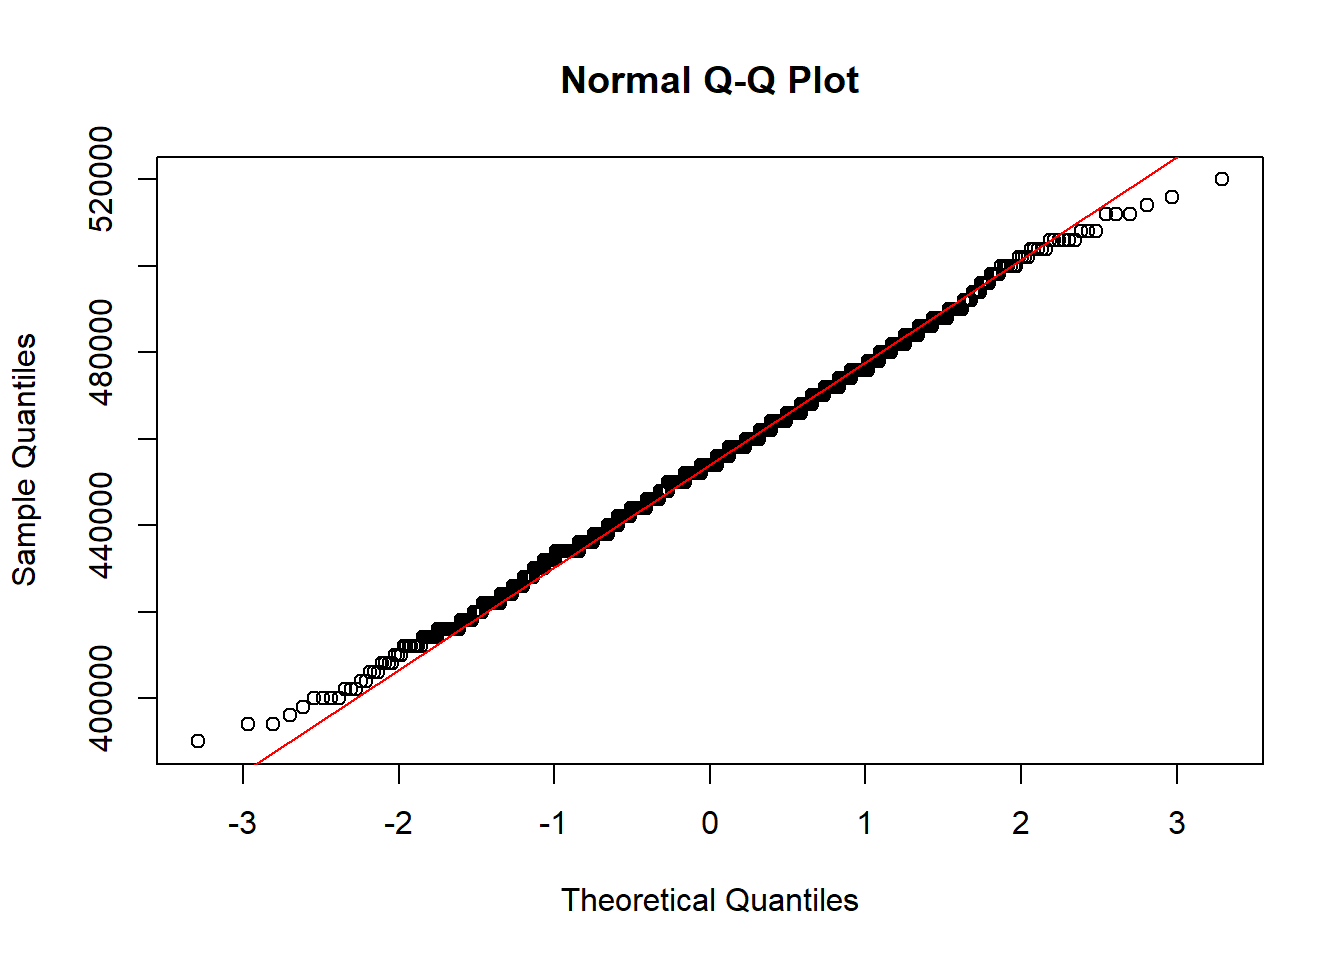
\includegraphics{ex1_files/figure-latex/unnamed-chunk-28-1.pdf}

\begin{Shaded}
\begin{Highlighting}[]
\CommentTok{#Salary vs math plot}
\KeywordTok{plot}\NormalTok{(}\DataTypeTok{x =}\NormalTok{ total}\OperatorTok{$}\NormalTok{salary, }\DataTypeTok{y =}\NormalTok{ total}\OperatorTok{$}\NormalTok{math_score, }\DataTypeTok{main =} \StringTok{"Salary vs. Math Score Plot"}\NormalTok{,}
     \DataTypeTok{ylab =} \StringTok{"Pisa math score"}\NormalTok{, }\DataTypeTok{xlab =} \StringTok{"Teachers salary"}\NormalTok{,}
     \DataTypeTok{pch =}\DecValTok{19}\NormalTok{, }\DataTypeTok{frame =} \OtherTok{FALSE}\NormalTok{)}
\end{Highlighting}
\end{Shaded}

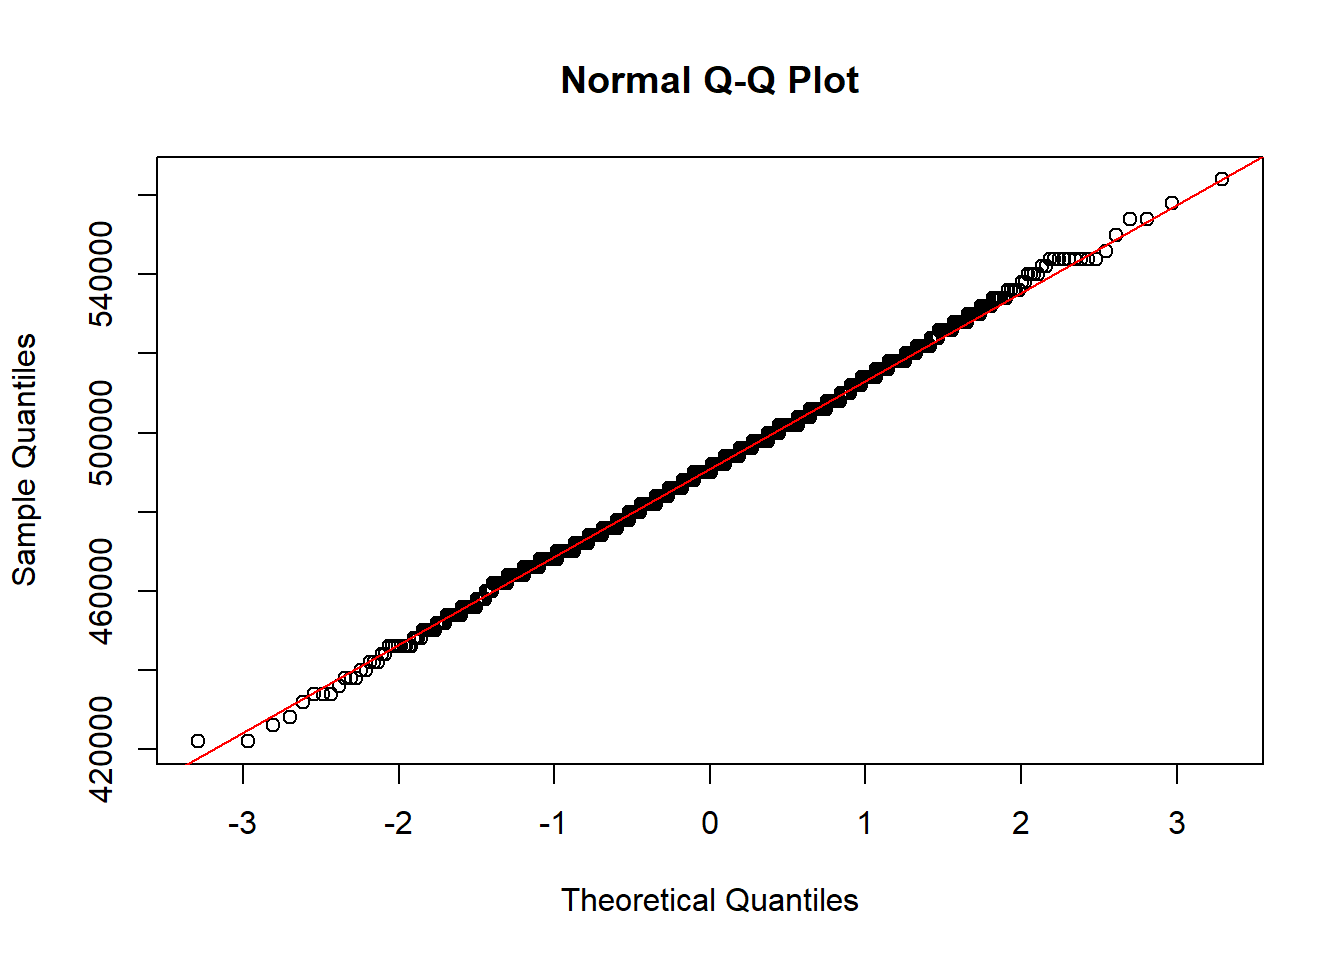
\includegraphics{ex1_files/figure-latex/unnamed-chunk-28-2.pdf}

\begin{Shaded}
\begin{Highlighting}[]
\CommentTok{#Salary vs science plot}
\KeywordTok{plot}\NormalTok{(}\DataTypeTok{x=}\NormalTok{ total}\OperatorTok{$}\NormalTok{salary, }\DataTypeTok{y =}\NormalTok{ total}\OperatorTok{$}\NormalTok{science_score, }\DataTypeTok{main =} \StringTok{"Salary vs. Science Score Plot"}\NormalTok{,}
     \DataTypeTok{ylab =} \StringTok{"Pisa science score"}\NormalTok{, }\DataTypeTok{xlab =} \StringTok{"Teachers salary"}\NormalTok{,}
     \DataTypeTok{pch =}\DecValTok{19}\NormalTok{, }\DataTypeTok{frame =} \OtherTok{FALSE}\NormalTok{)}
\end{Highlighting}
\end{Shaded}

\includegraphics{ex1_files/figure-latex/unnamed-chunk-28-3.pdf}

\begin{Shaded}
\begin{Highlighting}[]
\CommentTok{#Salary vs reading plot}
\KeywordTok{plot}\NormalTok{(}\DataTypeTok{x =}\NormalTok{ total}\OperatorTok{$}\NormalTok{salary, }\DataTypeTok{y =}\NormalTok{ total}\OperatorTok{$}\NormalTok{reading_score, }\DataTypeTok{main =} \StringTok{"Salary vs. Reading Score Plot"}\NormalTok{,}
     \DataTypeTok{ylab =} \StringTok{"Pisa reading score"}\NormalTok{, }\DataTypeTok{xlab =} \StringTok{"Teachers salary"}\NormalTok{,}
     \DataTypeTok{pch =}\DecValTok{19}\NormalTok{, }\DataTypeTok{frame =} \OtherTok{FALSE}\NormalTok{)}
\end{Highlighting}
\end{Shaded}

\includegraphics{ex1_files/figure-latex/unnamed-chunk-28-4.pdf}

\paragraph{3.4}\label{section-12}

\subparagraph{Conclusions}\label{conclusions}

We can see that there is some correlation between the teachers salary
and the grades. We can get some conclusions from those graphs. First, in
richer countries, where teachers earn more, it is possible that more
money was invested in education. It is also possible that students from
reacher countries has more tools to succeed, like private teachers or
after-hours classess. But, we can not forget that the data was collected
over more than 10 years, and for my opinion it is possible that the
teachers salary is getting higher every year beacause of Infaltion, and
that the grades are getting higher because more thecnology is envolved
this days in schools and students houses, thus a student can study math
or read more at home from various websites. In conclusion, for my
opinion the correlation is not strong enough, but it is possible that
there is a connection betwwen teachers salary and Pisa test, as written
above.

\paragraph{4.1}\label{section-13}

\subparagraph{Grades by region}\label{grades-by-region}

During the work on the grades tables, I was wondering if there is any
connection between geographic region and math grade. To do so, i decided
to color the world map by the Pisa math score value. And Here is the
results. More specifically, i decided to check regions around the
meditterenian sea. Here are the results:

\begin{Shaded}
\begin{Highlighting}[]
\NormalTok{twenty_six =}\StringTok{ }\NormalTok{data[}\KeywordTok{which}\NormalTok{(data}\OperatorTok{$}\NormalTok{year}\OperatorTok{==}\DecValTok{2006}\NormalTok{),]}
\NormalTok{twenty_six =}\StringTok{ }\KeywordTok{merge}\NormalTok{( salaries[(}\KeywordTok{which}\NormalTok{(}\KeywordTok{colnames}\NormalTok{(salaries)}\OperatorTok{==}\KeywordTok{c}\NormalTok{(}\StringTok{"Country"}\NormalTok{,}\StringTok{"2006"}\NormalTok{)))], twenty_six, }\DataTypeTok{by =} \KeywordTok{c}\NormalTok{(}\StringTok{"Country"}\NormalTok{) ,}\DataTypeTok{all =} \OtherTok{TRUE}\NormalTok{, }\DataTypeTok{sort =} \OtherTok{TRUE}\NormalTok{)}
\NormalTok{twenty_six =}\StringTok{ }\NormalTok{twenty_six[}\OperatorTok{-}\KeywordTok{c}\NormalTok{(}\DecValTok{5}\NormalTok{,}\DecValTok{13}\NormalTok{,}\DecValTok{74}\NormalTok{,}\DecValTok{75}\NormalTok{),]}
\NormalTok{twenty_six}\OperatorTok{$}\NormalTok{Country =}\StringTok{ }\NormalTok{(}\KeywordTok{trim}\NormalTok{(twenty_six}\OperatorTok{$}\NormalTok{Country))}


\NormalTok{twenty_nine =}\StringTok{ }\NormalTok{data[}\KeywordTok{which}\NormalTok{(data}\OperatorTok{$}\NormalTok{year}\OperatorTok{==}\DecValTok{2009}\NormalTok{),]}
\NormalTok{twenty_nine =}\StringTok{ }\KeywordTok{merge}\NormalTok{( salaries[(}\KeywordTok{which}\NormalTok{(}\KeywordTok{colnames}\NormalTok{(salaries)}\OperatorTok{==}\KeywordTok{c}\NormalTok{(}\StringTok{"Country"}\NormalTok{,}\StringTok{"2009"}\NormalTok{)))], twenty_nine, }\DataTypeTok{by =} \KeywordTok{c}\NormalTok{(}\StringTok{"Country"}\NormalTok{) ,}\DataTypeTok{all =} \OtherTok{TRUE}\NormalTok{, }\DataTypeTok{sort =} \OtherTok{TRUE}\NormalTok{)}
\NormalTok{twenty_nine =}\StringTok{ }\NormalTok{twenty_nine[}\OperatorTok{-}\KeywordTok{c}\NormalTok{(}\DecValTok{5}\NormalTok{,}\DecValTok{13}\NormalTok{,}\DecValTok{74}\NormalTok{,}\DecValTok{75}\NormalTok{),]}
\NormalTok{twenty_nine}\OperatorTok{$}\NormalTok{Country =}\StringTok{ }\NormalTok{(}\KeywordTok{trim}\NormalTok{(twenty_nine}\OperatorTok{$}\NormalTok{Country))}

\NormalTok{twenty_fifteen}\OperatorTok{$}\NormalTok{Country =}\StringTok{ }\NormalTok{(}\KeywordTok{trim}\NormalTok{(twenty_fifteen}\OperatorTok{$}\NormalTok{Country))}

\CommentTok{#create a map-shaped window}
\KeywordTok{mapDevice}\NormalTok{(}\StringTok{'x11'}\NormalTok{)}
\CommentTok{#join to a coarse resolution map}
\NormalTok{spdf <-}\StringTok{ }\KeywordTok{joinCountryData2Map}\NormalTok{(twenty_fifteen, }\DataTypeTok{joinCode=}\StringTok{"NAME"}\NormalTok{, }\DataTypeTok{nameJoinColumn=}\StringTok{"Country"}\NormalTok{)}
\NormalTok{spdf2 <-}\StringTok{ }\KeywordTok{joinCountryData2Map}\NormalTok{(twenty_six, }\DataTypeTok{joinCode=}\StringTok{"NAME"}\NormalTok{, }\DataTypeTok{nameJoinColumn=}\StringTok{"Country"}\NormalTok{)}
\NormalTok{spdf3 <-}\StringTok{ }\KeywordTok{joinCountryData2Map}\NormalTok{(twenty_nine, }\DataTypeTok{joinCode=}\StringTok{"NAME"}\NormalTok{, }\DataTypeTok{nameJoinColumn=}\StringTok{"Country"}\NormalTok{)}
\end{Highlighting}
\end{Shaded}

It is very interesting to see the changes along the years in european
countries, and how for example, countries like Germany Sweden and
Finland improved over the years, and the neighbours like spain and
portugal were left behind.

\begin{Shaded}
\begin{Highlighting}[]
\KeywordTok{mapCountryData}\NormalTok{(spdf2, }\DataTypeTok{nameColumnToPlot=}\StringTok{"math_score"}\NormalTok{, }\DataTypeTok{catMethod=}\StringTok{"fixedWidth"}\NormalTok{, }\DataTypeTok{colourPalette =} \StringTok{"diverging"}\NormalTok{, }\DataTypeTok{mapTitle =} \StringTok{"World Pisa math grades 2006"}\NormalTok{,  }\DataTypeTok{numCats =} \DecValTok{10}\NormalTok{, }\DataTypeTok{oceanCol =} \StringTok{"lightblue"}\NormalTok{, }\DataTypeTok{missingCountryCol =} \StringTok{"lightgrey"}\NormalTok{, }\DataTypeTok{mapRegion =} \StringTok{'Eurasia'}\NormalTok{, }\DataTypeTok{borderCol =} \StringTok{'black'}\NormalTok{)}
\end{Highlighting}
\end{Shaded}

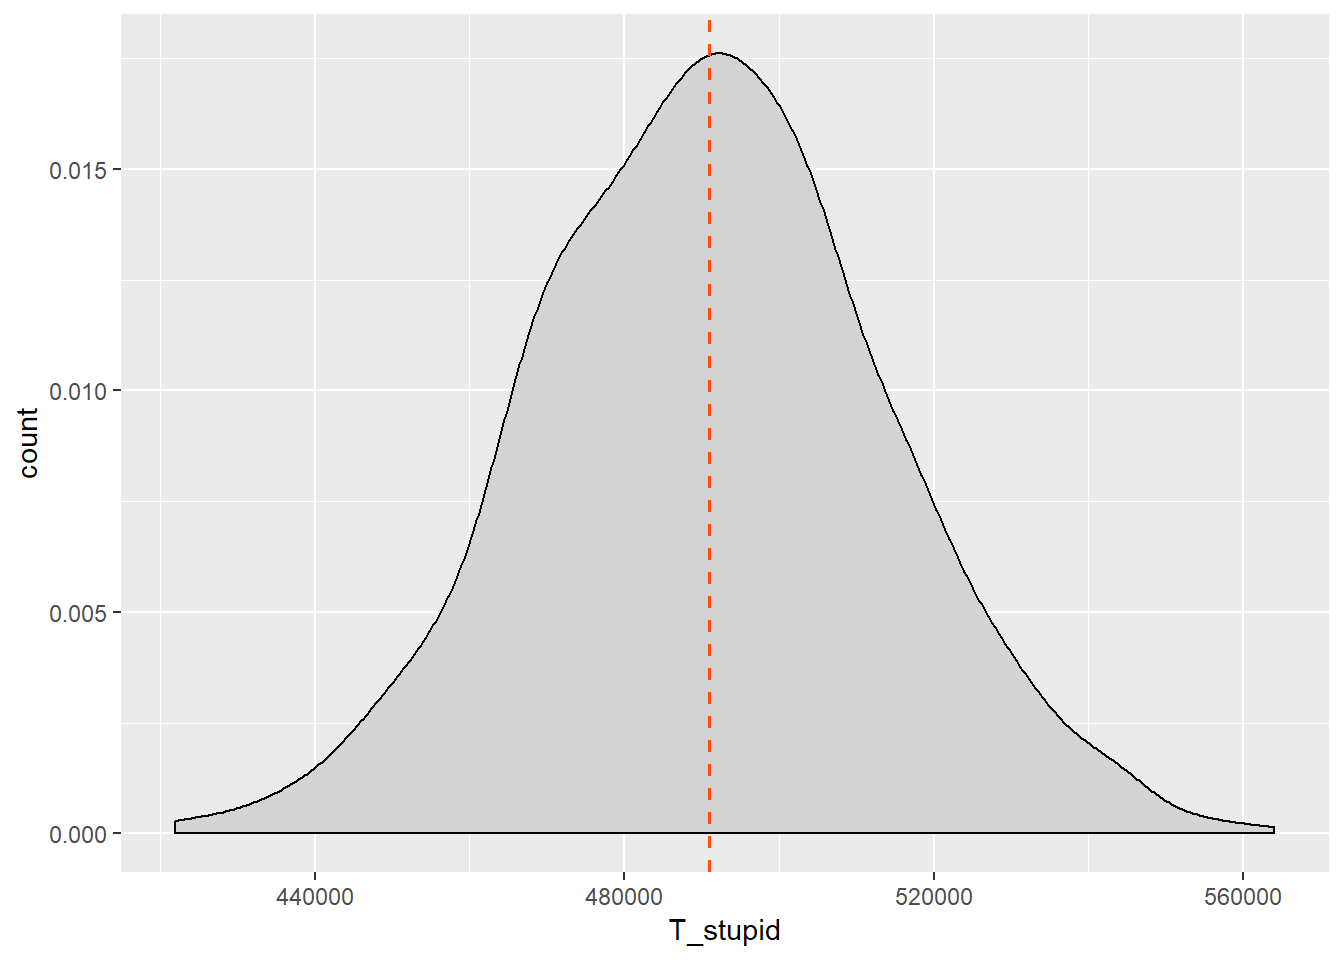
\includegraphics{ex1_files/figure-latex/unnamed-chunk-30-1.pdf}

\begin{Shaded}
\begin{Highlighting}[]
\KeywordTok{mapCountryData}\NormalTok{(spdf3, }\DataTypeTok{nameColumnToPlot=}\StringTok{"math_score"}\NormalTok{, }\DataTypeTok{catMethod=}\StringTok{"fixedWidth"}\NormalTok{, }\DataTypeTok{colourPalette =} \StringTok{"diverging"}\NormalTok{, }\DataTypeTok{mapTitle =} \StringTok{"World Pisa math grades 2009"}\NormalTok{, }\DataTypeTok{numCats =} \DecValTok{10}\NormalTok{, }\DataTypeTok{oceanCol =} \StringTok{"lightblue"}\NormalTok{, }\DataTypeTok{missingCountryCol =} \StringTok{"lightgrey"}\NormalTok{,}\DataTypeTok{mapRegion =} \StringTok{'Eurasia'}\NormalTok{, }\DataTypeTok{borderCol =} \StringTok{'black'}\NormalTok{)}
\end{Highlighting}
\end{Shaded}

\includegraphics{ex1_files/figure-latex/unnamed-chunk-30-2.pdf}

\begin{Shaded}
\begin{Highlighting}[]
\KeywordTok{mapCountryData}\NormalTok{(spdf, }\DataTypeTok{nameColumnToPlot=}\StringTok{"math_score"}\NormalTok{, }\DataTypeTok{catMethod=}\StringTok{"fixedWidth"}\NormalTok{, }\DataTypeTok{colourPalette =} \StringTok{"diverging"}\NormalTok{, }\DataTypeTok{mapTitle =} \StringTok{"World Pisa math grades 2015"}\NormalTok{, }\DataTypeTok{numCats =} \DecValTok{10}\NormalTok{, }\DataTypeTok{oceanCol =} \StringTok{"lightblue"}\NormalTok{, }\DataTypeTok{missingCountryCol =} \StringTok{"lightgrey"}\NormalTok{, }\DataTypeTok{mapRegion =} \StringTok{'Eurasia'}\NormalTok{, }\DataTypeTok{borderCol =} \StringTok{'black'}\NormalTok{)}
\end{Highlighting}
\end{Shaded}

\includegraphics{ex1_files/figure-latex/unnamed-chunk-30-3.pdf}

\paragraph{Special Thanks}\label{special-thanks}

\subsubsection{I would like to thanks Dr Yuval Benjamini from the Hebrew
Univuersity Jerusalem Institute for the data and all the questions asked
about
it.}\label{i-would-like-to-thanks-dr-yuval-benjamini-from-the-hebrew-univuersity-jerusalem-institute-for-the-data-and-all-the-questions-asked-about-it.}

\subsubsection{Special thanks to Mr.~Adi Ziv for the support and
guidance.}\label{special-thanks-to-mr.adi-ziv-for-the-support-and-guidance.}


\end{document}
